\chapter{Results}

\section{Said "What waht"}

\section{Winter tires}

\subsection{Fast track run}



\subsection{Two different mues}
The main goal for the work done in this report was to detect when low-$ \mu $ is present and thereafter be able to limit the torque transfer through the FXD. It is therefore essential to test the developed algorithm during a driving sequence that actually includes a changing $ \mu $. It has not been possible to test this on a single run, for example on asphalt and a skid pad. Therefore, two different runs have been merged together, where the friction coefficient changes three times.

The normalized force per slip ratio for this combined sequence can be seen in Figure \ref{slip_kraft_comb2}. Note that this figure is is merely Figure \ref{slip_kraft_ljungby} and \ref{slip_kraft_is} merged together, with some erroneous result when the friction coefficient changes come. 

\begin{figure}[h]
	\centering
	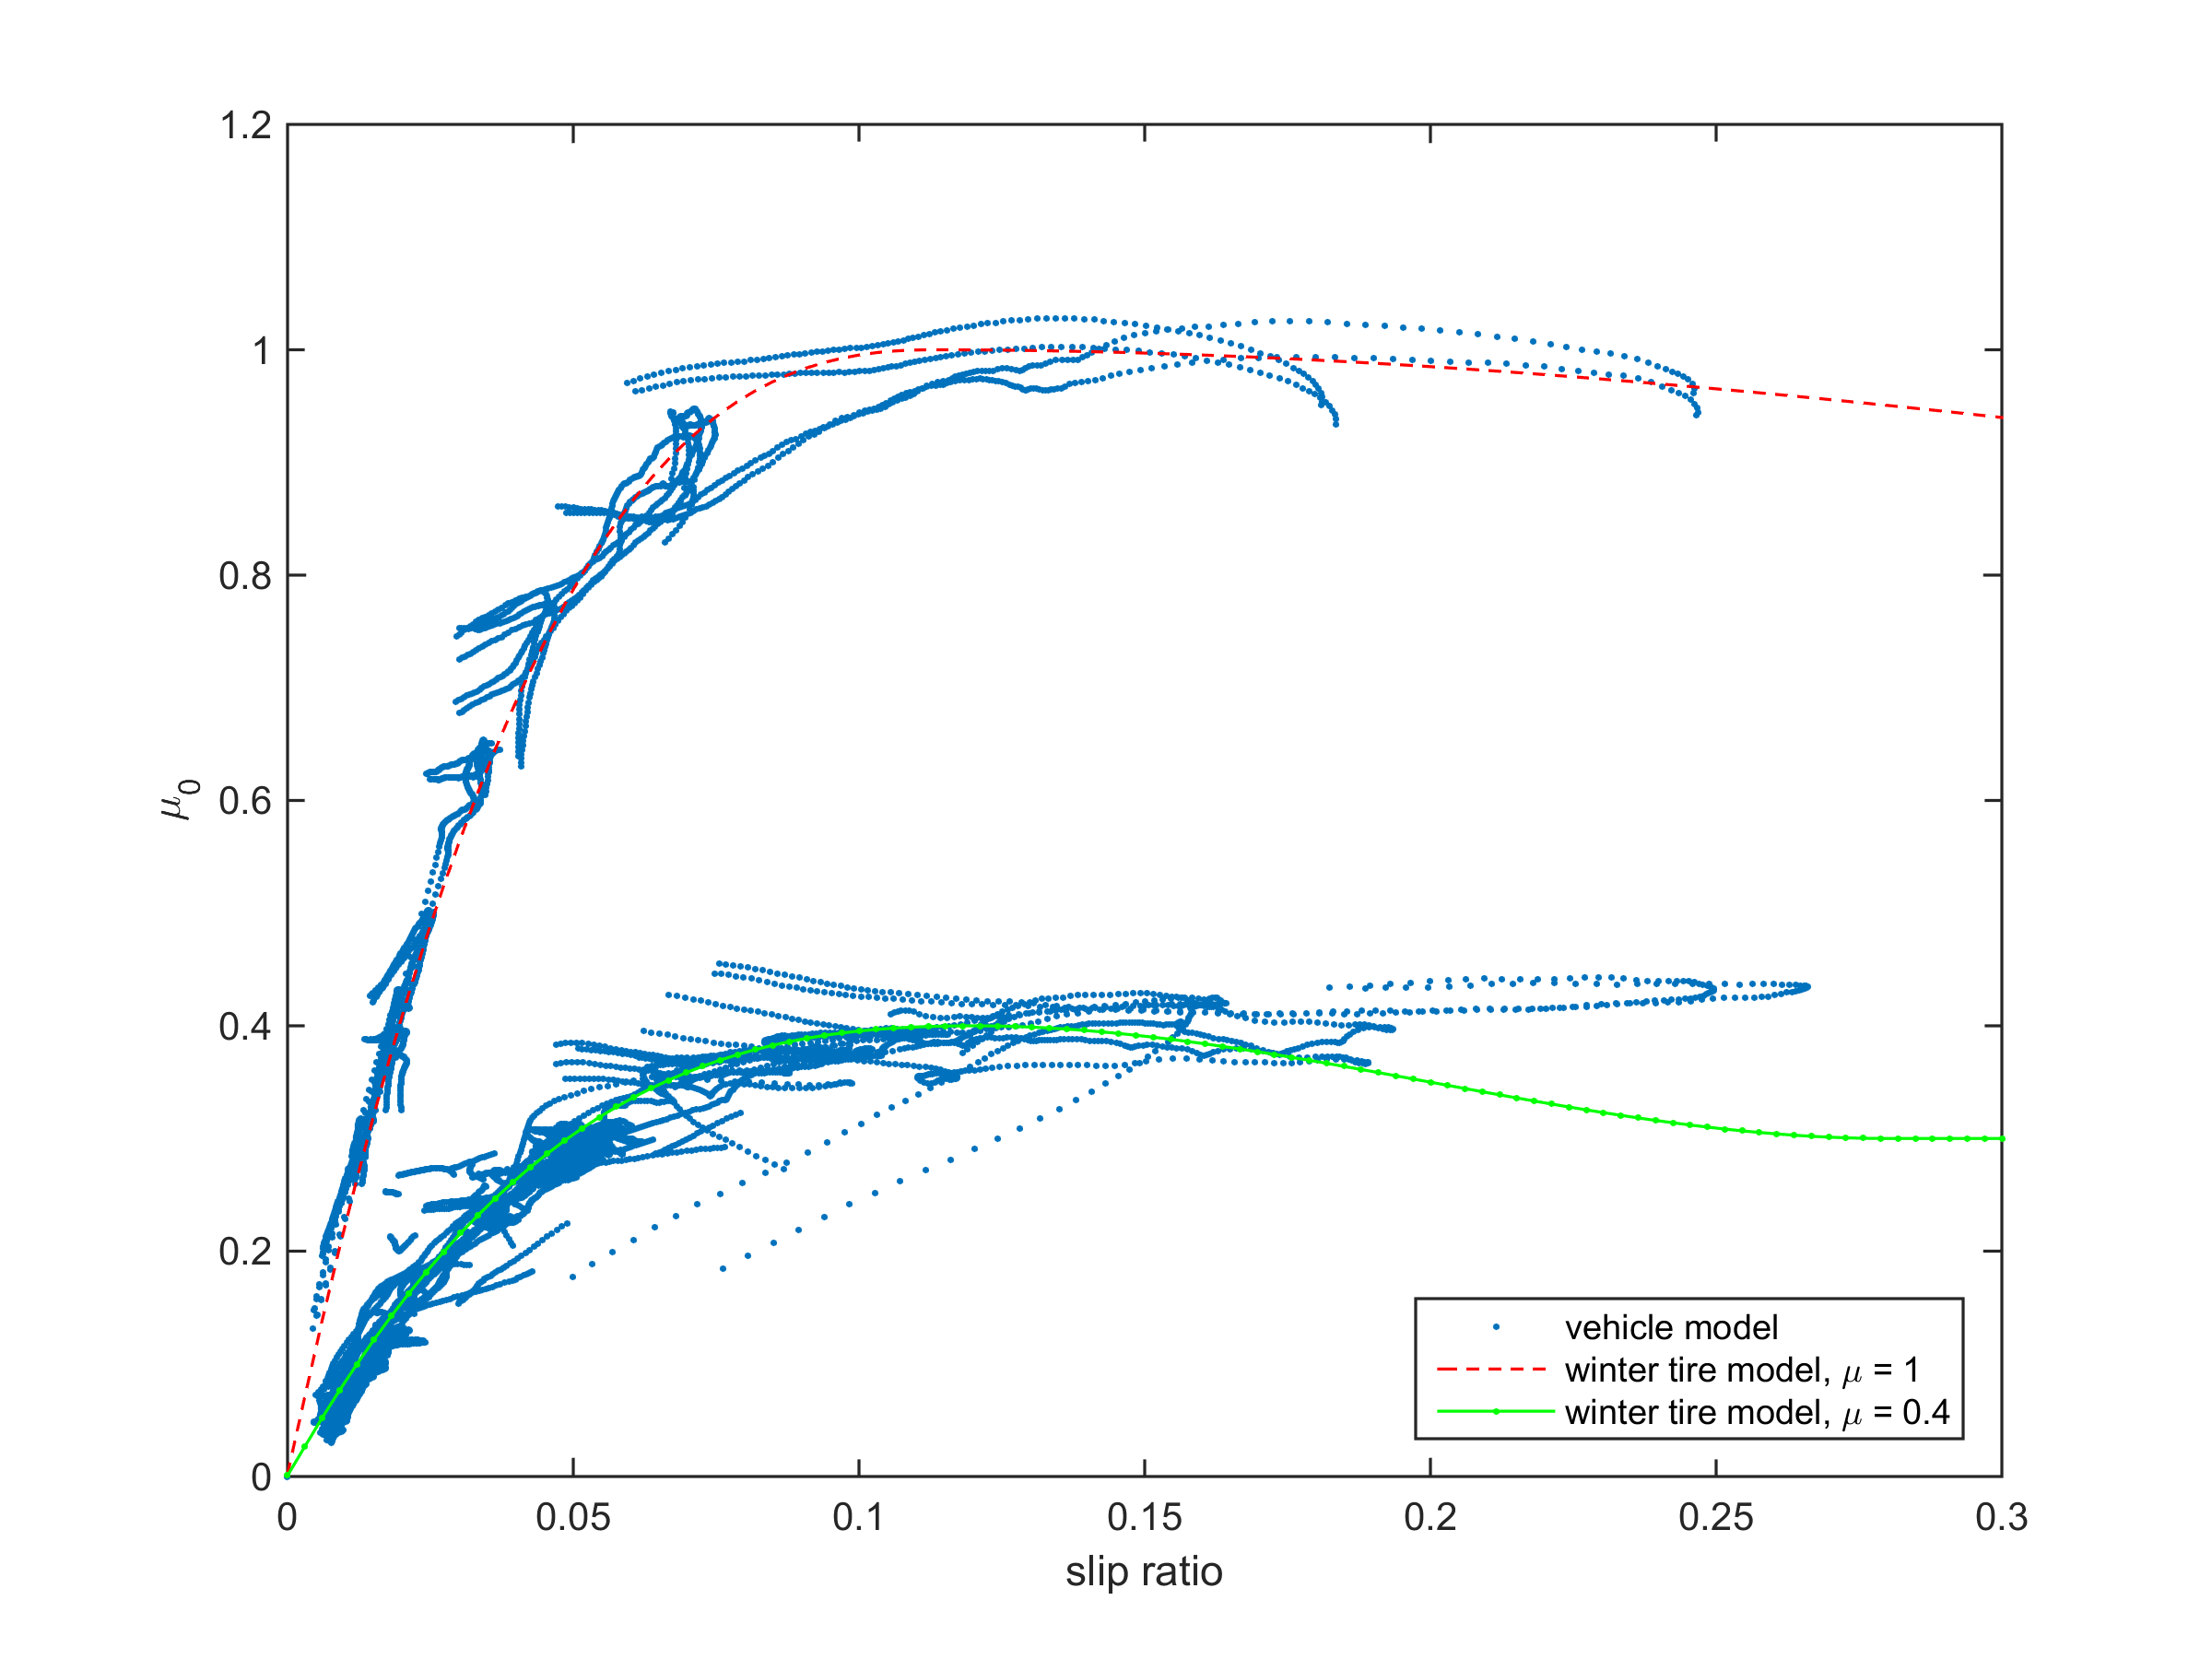
\includegraphics[width=1.0\textwidth]{Pictures/slip_kraft_comb2}
	\caption {Force per slip ratio for the combined driving sequence with both low- and high-$ \mu $.}
	\label{slip_kraft_comb2}
\end{figure}